\section{Integration of Concepts}
As explained in the previous section, we obtain maximised flux distribution of the metabolic organism for a single network state by performing linear optimisation. This section clarifies how the outputs from linear optimisation in more than one run are converted into a compatible format to construct data structures similar to {\color{red} real-life events}. With this integration step, one can construct association networks derived from FSS and FBS labels of the generated data and calculate modularity values concerning alternative null models.

 \begin{figure}[!ht]
	\begin{center}
		\makebox[\textwidth]{
			\centering
			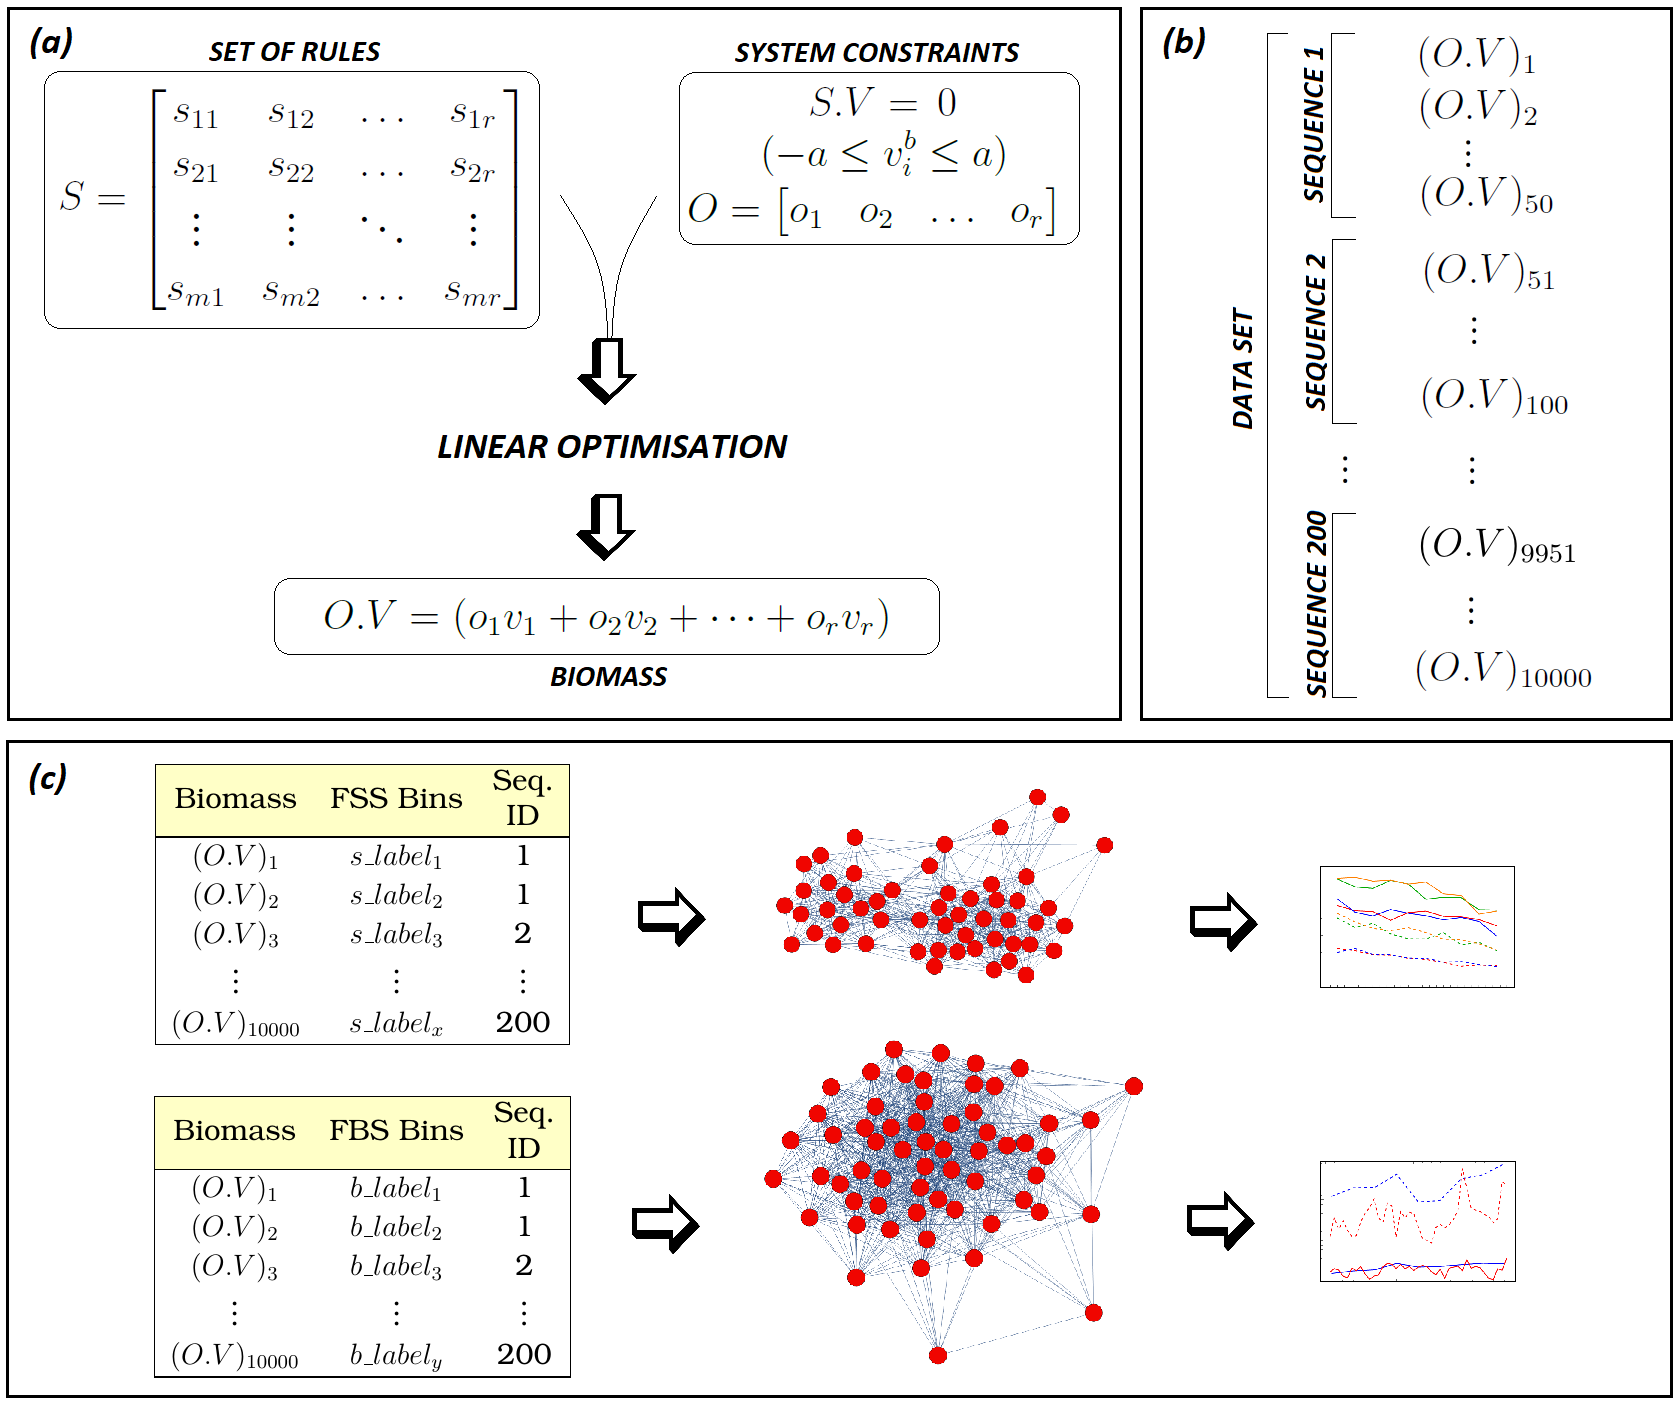
\includegraphics[width=1\linewidth]{../images/methodology-ORmodel-cartoon_complete_framework.png}}
		\caption{Simulation Model Illustration}
		\label{figure-complete_framework_cartoon}
	\end{center}
\end{figure}

%\begin{table}[hb!]
%	\centering
%	\setlength{\arrayrulewidth}{0.5pt}% 
%	\begin{tabular}{|ccc|}
%		\hline \rowcolor[HTML]{FFFFC7}
%		Biomass & FSS Bins	& \makecell{Seq.\\ID}  	\\ \hline
%		$(O.V)_{1}$	    & $s\_label_{1}$	& 1 		\\
%		$(O.V)_{2}$	    & $s\_label_{2}$	& 1 		\\
%		$(O.V)_{3}$	    & $s\_label_{3}$	& 2 		\\
%		\vdots  		& \vdots		& \vdots 	\\
%		$(O.V)_{10000}$	& $s\_label_{x}$	& 200 		\\ \hline
%	\end{tabular}
%\end{table}
%\begin{table}[hb!]
%	\centering
%	\setlength{\arrayrulewidth}{0.5pt}% 
%	\begin{tabular}{|ccc|}
%		\hline \rowcolor[HTML]{FFFFC7}
%		Biomass & FBS Bins	& \makecell{Seq.\\ID}  	\\ \hline
%		$(O.V)_{1}$	    & $b\_label_{1}$	& 1 		\\
%		$(O.V)_{2}$	    & $b\_label_{2}$	& 1 		\\
%		$(O.V)_{3}$	    & $b\_label_{3}$	& 2 		\\
%		\vdots  		& \vdots		& \vdots 	\\
%		$(O.V)_{10000}$	& $b\_label_{y}$	& 200 		\\ \hline
%	\end{tabular}
%\end{table}

%\begin{equation} %\tag{8}
%	(O.V)_{1}= (o_{1,1}v_{1} + o_{1,2}v_{2} + \dots + o_{1,r}v_{r})
%\end{equation}

%\begin{equation} %\tag{8}
%	(O.V)_{2}= (o_{2,1}v_{1} + o_{2,2}v_{2} + \dots + o_{2,r}v_{r})
%\end{equation}

%\begin{equation} 	
%	(O.V)_{50}= (o_{50,1}v_{1} + o_{50,2}v_{2} + \dots + o_{50,r}v_{r})
%\end{equation}

%\begin{equation} 	
%	(O.V)_{51}= (o_{1,1}v_{1} + o_{1,2}v_{2} + \dots + o_{1,r}v_{r})
%\end{equation}

%\begin{equation} 	
%	(O.V)_{100}= (o_{50,1}v_{1} + o_{50,2}v_{2} + \dots + o_{50,r}v_{r})
%\end{equation}

%\begin{equation} 	
%	(O.V)_{10000}= (o_{50,1}v_{1} + o_{50,2}v_{2} + \dots + o_{50,r}v_{r})
%\end{equation}

Fig.~\ref{figure-complete_framework_cartoon} illustrates the {\color{red}complete simulation model}. FBA optimisation scheme is summarised in Fig.~\ref{figure-complete_framework_cartoon}a with a defined set of rules and system constraints, as introduced in the previous section. The overall growth of the biomass (Eq.~\eqref{biomassmaximisation}) is obtained with a single run of the optimisation algorithm. The resultant value is a simulation event conceptually equivalent to a {\color{red} real-life production event}. The optimisation algorithm is run $10000$ times to create a data set with $10000$ events. 

Fig.~\ref{figure-complete_framework_cartoon}b shows the data structure generation by introducing a production sequence concept. {\color{red} Each sequence shows consistency among its production events}; therefore, the random choice for non-zero coefficients in the objective function is kept fixed only for the events in the same sequence. Hence, the optimisation scheme can use various fluxes to be considered in the biomass for created events in different sequences. 

Fig.~\ref{figure-complete_framework_cartoon}c shows the generated data labelled in alternative ways, as introduced in Tables~\ref{Tab: D-dataset-FSS} and \ref{Tab: D-dataset-FBS}, which is convenient to construct graphs to be analysed.